\documentclass[10pt]{amsart}
\usepackage{macros,slashed}

\linespread{1.25}

\usepackage{tikz}
\usetikzlibrary{arrows,shapes}
\usetikzlibrary{trees}
\usetikzlibrary{matrix,arrows}
\usetikzlibrary{positioning}
\usetikzlibrary{calc,through}
\usetikzlibrary{decorations.pathreplacing}
\usepackage{pgffor}

\def\sAd{\sA{\rm d}}

\usetikzlibrary{decorations.pathmorphing}
\usetikzlibrary{decorations.markings}
\tikzset{
	% >=stealth', %%  Uncomment for more conventional arrows
    vector/.style={decorate, decoration={snake}, draw},
	provector/.style={decorate, decoration={snake,amplitude=2.5pt}, draw},
	antivector/.style={decorate, decoration={snake,amplitude=-2.5pt}, draw},
    fermion/.style={draw=black, postaction={decorate},
        decoration={markings,mark=at position .55 with {\arrow[draw=black]{>}}}},
    fermionbar/.style={draw=black, postaction={decorate},
        decoration={markings,mark=at position .55 with {\arrow[draw=black]{<}}}},
    fermionnoarrow/.style={draw=black},
    gluon/.style={decorate, draw=black,
        decoration={coil,amplitude=4pt, segment length=5pt}},
    scalar/.style={dashed,draw=black, postaction={decorate},
        decoration={markings,mark=at position .55 with {\arrow[draw=black]{>}}}},
    scalarbar/.style={dashed,draw=black, postaction={decorate},
        dwecoration={markings,mark=at position .55 with {\arrow[draw=black]{<}}}},
    scalarnoarrow/.style={dashed,draw=black},
    electron/.style={draw=black, postaction={decorate},
        decoration={markings,mark=at position .55 with {\arrow[draw=black]{>}}}},
	bigvector/.style={decorate, decoration={snake,amplitude=4pt}, draw},
}

\usepackage[final]{pdfpages}

\title{}

\def\opp{{\rm op}}
\def\Ch{{\rm Ch}}
\def\dgLie{{\rm dgLie}}
\def\Lcat{L_\infty{\rm Alg}}
\def\Cur{{\rm Cur}}

\def\brian{\textcolor{blue}{BW: }\textcolor{blue}}


\begin{document}
\maketitle
\tableofcontents

\section{The holomorphic charge anomaly}

In this section, we switch gears a bit to propose a natural occurrence of the Kac-Moody factorization algebra as a symmetry of a simple class of higher dimensional quantum field theories. 
This situation is analogous to the free field realization of the affine Kac-Moody algebra as a subalgebra of a sort of Weyl algebra on the loop space. 

Our approach is through the general machinery of perturbative quantum field theory developed by Costello \cite{CosBook} and Costello-Gwilliam \cite{CG1,CG2}.
We study the quantization of a particular {\em free} field theory, which makes sense in any complex dimension.
Classically, the theory depends on the data of a $G$-representation, and the holomorphic nature of the theory allows us to lift this to a symmetry for the classical current algebra $\Cur^{\cl}(\sG_X)$ at ``zero level". 
We find that upon quantization, the symmetry is broken, but in a way that we can measure by an explicit anomaly, or cocycle. 
This leads to a symmetry of the theory via the quantum current algebra $\Cur^{\q}(\sG_X)$ twisted by this cocycle.  
 
%For any BV theory $\sE$, the BV operator $\{S,-\}$, which satisfies $\{S,-\}^2 =0$ by the ordinary classical master equation, together with the BV bracket $\{-,-\}$ equip the space of local functionals $\oloc(\sE)$ with the structure of a dg Lie algebra. 
%Another way to interpret the equivariant classical master equation is to view $I^{\sL}$ as an element in the dg Lie algebra $\oloc(\sE) \tensor \cloc^*(\sL)$.
%
%This section is mostly a cobbling together of know results above BV quantization for holomorphic theories found in the sources \cite{CG2, BWhol}. 
%
%%\subsection{The quantum master equation} 
%
%Suppose that $\fg$ is an ordinary Lie algebra that exists as a symmetry of a particular classical field theory. 

\subsection{Equivariant holomorphic matter}

We introduce a classical field theory in the BV formalism that one may think of as higher dimensional ``matter" in a holomorphic setting. 
When the complex dimension is $d = 1$, this returns the chiral $\beta\gamma$ system from ordinary conformal field theory. 
In dimensions $2$ and $4$, this theory is equal a minimal twist of supersymmetric matter. 

To start, we fix a finite dimensional $\fg$-module $V$ and an integer $d > 0$.
The classical fields of the complex $d$-dimensional theory consist of a map
\beqn\label{gammafield}
\gamma : \CC^d \to V
\eeqn
and a differential form of Hodge type $(d,d-1)$, $\beta \in \Omega^{d,d-1}(\CC^d, V^\vee)$ valued in the dual space $V^\vee$. 
The action functional describing the classical field theory is of the usual form
\beqn\label{actionfnl}
S(\gamma,\beta) = \int \<\beta, \dbar\gamma\>_V
\eeqn
where $\<-,-\>_V$ denotes the natural pairing between $V$ and its dual. 
The classical equations of motion of this theory consist of those $(\gamma,\beta)$ that are holomorphic, namely $\dbar \beta = \dbar \gamma = 0$. 

The symmetry we consider comes from the $\fg$-action on $V$. 
This extends, in a natural way, to an action of the gauge Lie algebra $C^\infty(\CC^d, \fg)$ on the fields (\ref{gammafield}): an element $X(z,\zbar) \in C^\infty(X,\fg)$ acts simply by $X(z,\zbar) \cdot \gamma(z,\zbar)$ where the dot indicates product of functions and the $\fg$-module structure on $V$. 
The condition that this action be compatible with the action functional (\ref{actionfnl}) says precisely that $X(z,\zbar)$ must be holomorphic: $\dbar X(z,\zbar) = 0$. 

Notice that the original action functional (\ref{actionfnl}) has an internal symmetry via the gauge transformation
\[
\beta \mapsto \beta + \dbar \beta' 
\]
where $\beta' \in \Omega^{d,d-2} (X, V^*)$. 
Thus, it is natural to include the space $\Omega^{d,d-2} (X, V^\vee)$ as the ghosts of the BRST formulation of this theory. 
Moreover, there are ghosts for ghosts $\beta'' \in \Omega^{d,d-3}(X , V^\vee)$, and so on.
Together with all of the antifields and antighosts, the full theory comprises of two copies of the Dolbeualt complex.
The precise definition is the following.

\begin{dfn}
The {\em classical $\beta\gamma$ system} on the complex manifold $X$, in the BV formalism, has space of fields
\[
\sE_V = \Omega^{0,*}(X , V) \oplus \Omega^{d,*}(X , V^*)[d-1],
\]
with the linear BRST operator given by $Q = \dbar$.
We will write fields as $(\gamma,\beta)$ to match with the notation above.
The $(-1)$-shifted symplectic pairing is given by integration along $X$ combined with the evaluation pairing between $V$ and its dual: $(\gamma, \beta) \mapsto \int_X \<\gamma, \beta\>_V$. 
The action functional for this free theory is thus
\[
S_V (\beta,\gamma) = \int_X \<\beta, \dbar \gamma\>_{V} .
\]
\end{dfn}

\begin{rmk}
As usual, the notation $[d-1]$ means we shift that copy of the fields down by $d-1$. 
Note that the elements in degree zero, where the physical fields live, are precisely maps $\gamma : Y \to V$ and sections $\beta \in\Omega^{d,d-1} (X ; V^\vee)$, just as in the description above. 
In this flat case the section $\beta$ has no dependence on $\gamma$.
the gauge symmetry $\beta \to \beta + \dbar \beta'$, where $\beta' \in \Omega^{d,d-2} (X, V^\vee)$ has naturally been incorporated into our BRST complex (which only consists of a linear operator since the theory is free).
\end{rmk}

By our discussion above, once we include the full BV complex, the symmetry by the Lie algebra $C^\infty(X, \fg)$ now extends to a symmetry by the {\em dg Lie algebra} $\sG_d^{sh} = \Omega^{0,*}(X, \fg)$. 
\brian{finish}

\begin{dfn/lem}
The $\sG_d$-equivariant $\beta\gamma$ system on $\CC^d$ with values in $V$ is defined by the local functional
\[
I^{\sG}(\alpha, \beta, \gamma) = \int \<\beta, \alpha \cdot \gamma\>_V \in \oloc(\sE_V \oplus \sG_d[1]) .
\]
This functional satisfies the $\sG_d$-equivariant classical master equation
\[
(\dbar + \d_{\sG}) I^{\sG} + \frac{1}{2} \{I^{\sG}, I^{\sG}\} = 0 .
\] 
\end{dfn/lem}

\subsubsection{The $\beta\gamma$ factorization algebra}

It is the general philosophy of \cite{CG1,CG2} that the observables of a quantum field theory form a factorization algebra on the underlying spacetime. 

%In this section we describe the factorization algebra associated to the higher $\beta\gamma$ system on $\CC^d$ associated to any $\fg$-representation $V$. 

%For any vector space $W$, we can consider the commutative algebra of algebraic and formal algebraic functions denoted respectively by
%\[
%\sO(W) = \Sym (W^\vee) = \bigoplus_{n \geq 0} (W^\vee)^{\tensor n}_{S_n} \;\;\; , \;\;\; \Hat{\sO}(W) = \Hat{\rm Sym}(W^\vee) %= \prod_{n \geq 0} (W^\vee)^{\tensor n}_{S_n} . 
%\] 

For any theory, the factorization algebra of classical observables assigns to every open set $U$ the cochain complex of algebraic functions on the fields supported on $U$.  
For the example of the $\beta\gamma$ system, the differential is just given by the $\dbar$ operator. 
Concretely, the complex of classical observables\footnote{There is also the completed version where one uses $\prod$ in place of $\oplus$ when defining the symmetric algebra, but we will not use it here.} assigned to an open set $U$ is
\[
\Obs^{\cl}_V(U) = \left(\Sym \left(\Omega^{0,*}(U)^\vee \tensor V^\vee \oplus \Omega^{d,*}(U)^\vee \tensor V [-d+1]\right), \dbar\right) .
\]
As usual, we use the completed tensor product when defining the symmetric products. 
It follows from the general results of Chapter 6 of \cite{CG2} that this assignment defines a factorization algebra on $\CC^d$. 

Upon taking global sections, the functional $I^{\sG}$ defines a map of dg Lie algebras $I^{\sG} : \sG_d(\CC^d) \to \Obs^{\cl}_V(\CC^d)$.
We have seen that $\Obs_V^{\cl}$ is a factorization algebra equipped with a $P_0$-structure. 
In the introduction, we also discussed how a local Lie algebra determines a $P_0$-factorization algebra via its classical current algebra. 
The classical Noether's theorem, as proved in Chapter 11 of \cite{CG2}, says that $I^{\sG}$ determines a map between these factorization algebras. 

\begin{prop}{\cite{[CG2]}} (Classical Noether's Theorem)
The assignment that sends an element $\alpha \in \Omega^{0,*}_c(U, \fg)$ to the observable
\[
\gamma \tensor \beta \in \Omega^{0,*}(U, V) \tensor \Omega^{d,*}(U, V^*) \mapsto \int_U \<\beta, \alpha \cdot \gamma\>_V
\]
determines a map of $P_0$-factorization algebras on $\CC^d$
\[
J^{\cl} : \Cur^{\cl} (\sG_d) \to \Obs^{\cl}_V .
\]
\end{prop}

\begin{rmk}
The formula for $J^{\cl}$ is identical to that of the local functional $I^\fg(\alpha)$ defining the action of $\sG_d$ on the $\beta\gamma$ system.
Ordinarily, a local functional does not determine an observable on an open set since the integral may not exist.
However, since $\alpha$ is compactly supported on $U$, it makes sense to restrict $I^\sG (\alpha)$ to an observable on $U$. 
This is precisely the observable $J^{\cl}(\alpha)$. 
\end{rmk}

As usual, the statement we are after pertains to the quantum situation. 
Being a free field theory, the $\beta\gamma$ system admits a unique quantization and hence a factorization algebra $\Obs^{\q}_V$ of quantum observables (whose definition we recall below). 
The natural question arises whether the symmetry by the dg Lie algebra $\sG_d$ persists upon quantization. 
We are asking if we can lift $J^{\cl}$ to a ``quantum current" $J^{\q} : \Cur^\q(\sG_d) \to \Obs^\q_V$, where $\Cur^\q(\sG_d)$ is the factorization algebras of quantum currents defined in the introduction. 
The existence of this map of factorization algebras is controlled by the equivariant quantum master equation, which we now turn to.

\subsection{The equivariant quantization}

The approach to quantum field theory we use follows Costello's theory of renormalization and the Batalin-Vilkovisky formalism developed in \cite{CosRenorm}.
The formalism dictates that in order to define a quantization, it suffices to define the theory at each energy (or length) scale and to ask that these descriptions be compatible as we vary the scale.
Concretely, this compatibility is through the {\em renormalization group (RG) flow} and is encoded by an operator $W(P_{\epsilon < L}, -)$ acting on the space of functionals. 
The functional $W(P_{\epsilon < L},-)$ is defined as a sum over weights of graphs which is how Feynman diagrams appear in Costello's formalism.
A theory that is compatible with the RG flow is called a ``prequantization". 
In order to obtain a quantization, one must solve the quantum master equation (QME). 
For us, the quantum master equation encodes the failure of lifting the classical $\sG_d$-symmetry to one on the prequantization.

The quantization we work with follows Costello's general approach very closely, with the slight caveat that we are working equivariantly, and so some of the fields are actually background fields. 
The two main ingredients to construct the weight are the propagator $P_{\epsilon < L}$ and the classical interaction $I^{\sG}$. 
The propagator only depends on the underlying free theory, that is, the higher dimensional $\beta\gamma$ system. 
For the general definition, we refer the reader to can be found in Section ?? of \cite{CG2}.
As above, the interaction describes how the linear currents $\sG_d$ act on the free theory. 

The construction of $P_{\epsilon<L}$, which makes sense for a wide class theories of this holomorphic flavor, can be found in Section 3.2 of \cite{BWhol}.
For us, it is important to know that $P_{\epsilon<L}$ satisfies the following properties:

\begin{enumerate}
\item[(1)] For $0 < \epsilon < L < \infty$ the propagator is a symmetric element
\[
P_{\epsilon < L} \in \sE_V \Hat{\tensor} \sE_V .
\]
Moreover, $P_{0 < \infty} = \lim_{\epsilon \to 0}\lim_{L \to \infty}$ is a symmetric element of the distributional completion $\Bar{\sE}_V \Hat{\tensor} \Bar{\sE}_V$. 

\item[(2)] 
The propagator lies in the subspace
\[
\Omega^{d,*}(\CC^d \times \CC^d, V \tensor V^*) \oplus \Omega^{d,*}(\CC^d \times \CC^d, V^* \tensor V) \subset \sE_V \Hat{\tensor} \sE_V .
\]
If we coordinatize $(z,w) \in \CC^d \times \CC^d$, the propagator has the form
\beqn
P_{\epsilon<L} = P^{an}_{\epsilon<L}(z,w) \tensor \left({\rm id}_{V} + {\rm id}_{V^*}\right)
\eeqn
where ${\rm id}_V, {\rm id}_{V^*}$ are the elements representing the identity maps which lie in $V \tensor V^*, V^* \tensor V$ respectively. 
Moreover, $P^{an}_{0 < \infty} (z,w)$ is the Green's function for the Hodge Laplacian $\triangle_{\rm Hodge}$ on $\CC^d$:
\[
\triangle_{\rm Hodge} P^{an}_{0<\infty} (z,w) = \delta (z-w) .
\]

\item[(3)] Let $K_t \in C^\infty((0,\infty)_t) \tensor \sE_V \Hat{\tensor} \sE_V$ be the heat kernel for the Hodge Laplacian
\[
\triangle_{\rm Hodge} K_t + \frac{\partial}{\partial t} K_t = 0 .
\]
Then, $P_{\epsilon < L}$ provides a $\dbar$-homotopy between $K_\epsilon$ and $K_L$:
\[
\dbar P_{\epsilon < L} = K_{t=L} - K_{t=\epsilon} .
\]
\end{enumerate}

%The building block in Costello's approach to renormalization is an effective family of functionals $\{I[L]\}$ parametrized by a {\em length scale} $L > 0$. 
%For each $L > 0$ the functional $I[L] \in \sO(\sE)[[\hbar]]$ must satisfy various conditions, which are carefully stated in Definition 8.2.9.1 of \cite{CG2}. 
%We will recall some key aspects that will be useful for our purposes. 
%The main condition is a compatibility between the functionals $I[L]$ as one changes the length scale; this is referred to as {\em homotopy renormalization group (RG) flow}.

To define the quantization, we must recall the definition of a weight of a Feynman diagram adjusted to this equivariant context.
To simplify our discussion, we introduce the notation $\sO(\sG_d[1])$ to mean the underlying graded vector space of $\clie^*(\sG_d)$, so the symmetric algebra on the dual of $\sG_d$. 

For the free $\beta\gamma$ system, the homotopy RG flow from scale $L>0$ to $L'>0$ is an invertible linear map 
\beqn\label{weight1}
W(P_{L < L'} , -) : \sO(\sE) [[\hbar]] \to \sO(\sE)[[\hbar]]
\eeqn
defined as a sum over weights of graphs $W (P_{L<L'}, I) = \sum_{\Gamma} W_{\Gamma}(P_{L<L'}, I)$. 
Here, $\Gamma$ denotes a graph, and the weight $W_\Gamma$ associated to $\Gamma$ is defined as follows.
One labels the vertices of valence $k$ by the $k$th homogenous component of the functional $I$. 
The edges of the graph are labeled by the propagator $P_{L<L'}$.
The total weight is given by iterative contractions of the homogenous components of the interaction with the propagator. 
Formally, we can write the weight as
\[
e^{W(P_{\epsilon <L}, I)} = e^{\hbar \partial_{P_{\epsilon <L}}} e^{I / \hbar}
\]
where $\partial_P$ denotes contraction with $P$. 
For a more precise definition see Chapter 2 of \cite{CosRenorm}.

To define the equivariant version, we extend (\ref{weight1}) to a $\sO(\sG_d[1])$-linear map
\[
W^{\sG} (P_{L < L'} , -) : \sO(\sE \oplus \sG_d[1]) [[\hbar]] \to \sO(\sE \oplus \sG_d[1])[[\hbar]] .
\]

\begin{dfn/lem}
The {\em prequantization} of the $\sG_d$-equivariant $\beta\gamma$ system on $\CC^d$ is defined by the family of functionals $\{I^{\sG}[L]\}_{L > 0}$, where
\beqn\label{prequant}
I^{\sG} [L] = \lim_{\epsilon \to 0} W^{\sG} (P_{\epsilon<L} , I^{\sG}) .
\eeqn 
This family satisfies homotopy RG flow and solves the quantum master equation modulo $\cloc^*(\sG_d)$. 
\end{dfn/lem}

\begin{proof}
The non-trivial claim to justify here is why the $\epsilon \to 0$ limit of $W^{\sG} (P_{\epsilon<L} , I^{\sG})$ exists. 
This follows from the following two claims:

\begin{itemize}
\item[(1)] 
Only one-loop graphs appear in the weight expansion $W^{\sG} (P_{\epsilon < L}, I^{\sG})$. 

\item[(2)] Let $\Gamma$ be a one-loop graph.
Then
\[
\lim_{\epsilon \to 0} W^{\sG}_\Gamma(P_{\epsilon < L}, I^{\sG})
\]
exists.
\end{itemize}

First, we justify claim (1).
Recall that the weight is defined as a sum over {\em connected} graphs.
An immediate consequence of the combinatorics involved in constructing the equivariant weight using the $\beta\gamma$ propagator \brian{finish}. 



\end{proof}

As an immediate consequence of the proof, we see that only polynomial values of $\hbar$ occur in the expansion of $I^{\sG}[L]$. 
This fact will be used later on when we make sense of the ``free field realization" of the Kac-Moody granted by this equivariant quantization. 

\begin{cor}
For each $L > 0$, the functional $I^{\sG}[L]$ lies in the subspace $\sO(\sE \oplus \sG_d[1]) [\hbar] \subset \sO(\sE \oplus \sG_d[1]) [[\hbar]]$. 
\end{cor}

To define the quantum master equation, we must introduce the BV Laplacian $\Delta_L$ and the scale $L$ BV bracket $\{-,-\}_L$. 
For $L > 0$, the operator $\Delta_L : \sO(\sE_V) \to \sO(\sE_V)$ is defined by contraction with the heat kernel $K_L$ defined above. 
Similarly, $\{-,-\}_L$ is a bilinear operator on $\sO(\sE_V)$ defined by
\[
\{I,J\}_L = \Delta_L(IJ) - (\Delta_L I)J - (-1)^{|I|} I \Delta_L J .
\] 
There are equivariant version of each of these operators given by extending via $\sO(\sG_d[1])$-linearity.
For instance, the BV Laplacian is a degree one operator of the form
\[
\Delta_L : \sO(\sE \oplus \sG_d[1]) \to \sO(\sE \oplus \sG_d[1]) .
\]
We say a functional $J \in \sO(\sE_V \oplus \sG_d[1])$ satisfies the scale $L$, $\sG_d$-{\em equivariant quantum master equation} if
\[
(\dbar + \d_{\sG}) J+ \frac{1}{2} \{J, J\}_L + \hbar \Delta_L J = 0 .
\]
The main object of study in this section is the failure for the quantization $I^{\sG}[L]$ to satisfy this equivariant QME. 

\begin{dfn}
The scale $L$, $\sG_d$-{\em equivariant charge anomaly} is
\[
\hbar \Theta_V [L] = (\dbar + \d_{\sG}) I^{\sG} [L] + \frac{1}{2} \{I^{\sG}[L], I^{\sG}\}_L + \hbar \Delta I^{\sG}[L] .
\]
As above, $\d_{\sG}$ denotes the Chevalley-Eilenberg differential $\clie^*(\sG_d) = \left(\sO(\sG_d[1]), \d_{\sG}\right)$. 
\end{dfn}

\subsection{The charge anomaly for $\beta\gamma$}

To calculate the anomaly to solving the $\sG_d$-equivariant master equation we utilize a general result about the quantum master equation for holomorphic field theories formulated in \cite{BWhol}. 
In general, since the effective field theory defining the prequantization $\{I^{\sG}[L]\}$ is given by a Feynman diagram expansion, the anomaly to solving the quantum master equation is also given by a potentially complicated sum of diagrams. 
As an immediate corollary of Proposition 4.4 of \cite{BWhol} for holomorphic theories on $\CC^d$, we find that only a simple class of diagrams appear in the anomaly. 

\begin{lem}\label{lem: obs}
Let $\Theta_V[L]$ be the $\sG_d$-{\em equivariant charge anomaly} for the $\beta\gamma$ system with values in $V$.
Then, $\Theta_V := \lim_{L \to 0} \Theta_V[L]$ exists, and is a local cocycle 
\[
\Theta_V \in \cloc^*(\sG_d) .
\]
Furthermore, $\Theta$ is computed by the following limit
\[
\hbar \Theta_V = \frac{1}{2} \lim_{L \to 0} \lim_{\epsilon \to 0} \sum_{\Gamma \in {\rm Wheel}_{d+1} \; , e} W_{\Gamma, e}(P_{\epsilon <L}, K_\epsilon, I^{\sG}) ,
\] 
where the sum is over all wheels of valency $(d+1)$ and internal edges $e$. 
\end{lem}

\begin{figure}
\begin{center}
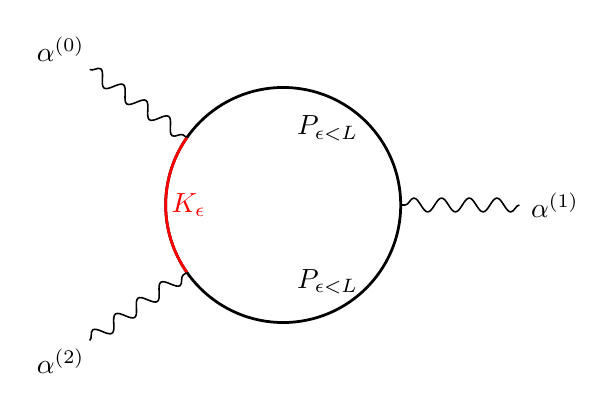
\begin{tikzpicture}[line width=.2mm, scale=1.5]

%\pgfmathsetmacro{\ex}{0}
%\pgfmathsetmacro{\ey}{1}

%\draw (\ex,\ey) ++(45:.8) arc (45:-45:.8);

		\draw[fill=black] (0,0) circle (1cm);
		%\draw[fill=red] (0,0) arc (145:215:1);
		\draw[fill=white] (0,0) circle (0.99cm);
		\draw[line width=0.35mm,red] ++(145:0.995) arc (145:215:0.995);
		%\draw[red] (0,0) arc (30:60:3);

		\draw[vector](145:2) -- (145:1);
		\node at (145:2.3) {$\alpha^{(0)}$};
			%\node at (145:0.85) {$v_0$};
		\node at (60:0.75) {$P_{\epsilon<L}$};
		\node at (-60:0.75) {$P_{\epsilon<L}$};
		\draw[vector](215:2) -- (215:1cm);
		\node at (215:2.3) {$\alpha^{(2)}$};
			%\node at (215:0.85) {$v_{d}$};
		\node[red] at (180:0.8) {$K_\epsilon$};
		\draw[vector](0:2) -- (0:1);
		\node at (0:2.3) {$\alpha^{(1)}$};
			%\node at (35:0.85) {$v_{\alpha}$};
		%\node at (0:0.8) {$P_{\epsilon<L}$};
		%\node at (270:0.8) {$P_{\epsilon<L}$};
	    	\clip (0,0) circle (1cm);
\end{tikzpicture}
\caption{The diagram representing the weight $W_{\Gamma, e}(P_{\epsilon<L}, K_\epsilon, I^\fg)$ in the case $d=2$. 
On the black internal edges are we place the propagator $P_{\epsilon < L}$ of the $\beta\gamma$ system. 
On the red edge labeled by $e$ we place the heat kernel $K_\epsilon$.
The external edges are labeled by elements $\alpha^{(i)} \in \Omega^{0,*}_c(\CC^2)$.}
\label{fig:liewheel}
\end{center}
\end{figure}

\begin{rmk}
If $\Gamma$ is a graph with a distinguished edge $e$ and $A,B$ are elements of the tensor square of fields $A, B \in \sE \tensor \sE$, we let $W_{\Gamma,e}(A,B, I)$ denotes the weight of the graph where we place $B$ at the internal edge labeled $e$ and $A$ on the remaining internal edges.
\end{rmk}

In the remainder of this section we will characterize this anomaly algebraically, using the identification of Proposition \cite{prop: trans j}. 
Actually, it is immediate based on symmetry arguments what the obstruction is up to a scalar multiple. 

First, we note that the element $\Theta_V \in \cloc^*(\sG_d)$ lifts to the invariant subspace of $U(d)$-invariant, holomorphic translation invariant local cocycles.
This follows from the fact that both the functional $I^{\sG}$ and propagator $P_{\epsilon<L}$ are $U(d)$-invariant, holomorphic translation invariant.
By Proposition \ref{prop: trans j} we see that $\Theta_V$ must be cohomological to a cocycle of the form
\[
(\alpha_0, \ldots, \alpha_d) \mapsto \int_{\CC^d} \theta(\alpha_0 \wedge \partial \alpha_1 \wedge \cdots \wedge \partial \alpha_d) 
\]
where $\theta$ is some element of $\Sym^{d+1}(\fg^*)^\fg$.
In the notation of Section \ref{??}, this is the cocycle $\fJ_d (\theta)$. 
This cocycle factors in the following way:
\beqn\label{composition}
\begin{tikzcd}
\left(\Omega^{0,*}_c(\CC^d) \tensor \fg\right)^{\tensor (d+1)} \ar[r,"\fa \fn"] & \left(\Omega^{0,*}_c(\CC^d) \tensor \fg\right) \tensor \left(\Omega^{1,*}_c(\CC^d)\tensor \fg\right)^{\tensor d} \ar[r, "\theta"] & \Omega^{d, *}_c(\CC^d) \ar[r, "\int"] & \CC . 
\end{tikzcd}
\eeqn
The first map is $\fa \fn : \alpha_0 \tensor \cdots \tensor \alpha_d \mapsto \alpha_0 \tensor \partial \alpha_1 \tensor \cdots \tensor \partial \alpha_d$.
The second map is given by extending the Lie algebraic functional $\theta : \fg^{\tensor (d+1)} \to \CC$ to the Dolbeault complex in the obvious way:
\[
\theta \left(\alpha_0 \tensor (\alpha_1 \tensor \cdots \tensor \alpha_d\right) = \alpha_0 \wedge \theta(\alpha_1 \wedge \cdots \wedge \alpha_d) \in \Omega^{d,*}_c(\CC^d).
\]

Lemma \ref{lem: obs} implies that the obstruction is given by the sum over Feynman weights associated to graphs of wheels of valency $(d+1)$.
We can identify the algebraic component, corresponding to $\theta$ in the above composition (\ref{composition}), directly from the shape of this graph. 
The propagator and heat kernel $P_{\epsilon<L}, K_\epsilon$ labeling the edges factor as
\[
P_{\epsilon<L} = P^{an}_{\epsilon<L} \tensor \left({\rm id}_{V} + {\rm id}_{V^*}\right) \;\; , \;\; K_{\epsilon} = K_{\epsilon}^{an} \tensor \left({\rm id}_{V} + {\rm id}_{V^*}\right)
\]
where ${\rm id}_V, {\rm id}_{V^*}$ are the elements representing the identity maps which lie in $V \tensor V^*, V^* \tensor V$ respectively. 
The analytic factors $P^{an}_{\epsilon<L},  K_{\epsilon}^{an}$ only depend on the dimension $d$. 

Each trivalent vertex of the wheel is also labeled by both an analytic factor and Lie algebraic factor. 
The Lie algebraic part of each vertex can be thought of as the defining map of the representation $\rho : \fg \to {\rm End}(V)$. 
The diagrammatics of the wheel amounts to taking the trace of the symmetric $(d+1)$st power of this Lie algebra factor. 
Thus, the Lie algebraic factor of the weight of the wheel is the $(d+1)$st component of the character of the representation
\[
{\rm ch}_{d+1}^\fg(V) = \frac{1}{(d+1)!} {\rm Tr}\left(\rho(X)^{d+1}\right) \in \Sym^{d+1}(\fg^*) .
\]

By these symmetry arguments, we know that the anomaly will be of the form $\Theta = A \fj (\ch_{d+1}^{\fg}(V))$ for some number $A \in \CC$.
In Appendix \ref{sec: feynman}, we perform an explicit calculation of this constant $A$, which depend on the specific form of the analytic propagator and heat kernel. 
We arrive at the following.

\begin{prop}\label{prop: bg anomaly}
The charge anomaly for quantizing the $\sG_d$-equivariant $\beta\gamma$ system on $\CC^d$ is equal to
\[
\Theta_V = A  \fj (\ch_{d+1}^{\fg}(V)),
\]
where $\fj$ is the isomorphism from Proposition \ref{prop: trans j}.
\end{prop}

\subsection{The quantum observables of the $\beta\gamma$ system}

Before deducing the main consequence of the anomaly calculation, we introduce the quantum observables of the $\beta\gamma$ system. 
The quantum observables $\Obs^{\q}_V$ define a quantization of the classical observables in the sense that there is an isomorphism
\[
\Obs^{\cl}_V \cong \Obs^\q_V \tensor_{\CC[\hbar]} \CC_{\hbar = 0} .
\]
In practice, the BV formalism suggests that the quantum observables arise by 
\begin{enumerate}
\item[(a)] tensoring the underlying graded vector space of $\Obs^\cl_n$ with $\CC[[\hbar]]$ and
\item[(b)] deforming the differential to $\dbar +\hbar \Delta_L$, where $\Delta_L$ is the BV Laplacian.
\end{enumerate}
This actually defines a family of quantum observables, one for each length scale $L$. 
A main idea of \cite{CG2} says that by considering the collection of functionals at all length scales $L$, the observables $\Obs^\q_V$ still define a factorization algebra. 

The fact that this works is quite subtle, since naively the differential $\Delta_L$ seems to have support on all of $\CC^d$, so it's not obvious how to define the corestriction maps of the factorization algebra. 
In the case of free theories, such as the $\beta\gamma$ system, there is a way to circumvent this difficulty. 
One can work with a smaller class of observables --- such as those arising from smooth functionals, not distributional ones.
Then, one can make sense of the limit $\Delta = \lim_{L \to 0} \Delta_L$, and just use this single BV Laplacian. 
This approach is developed in detail for the free $\beta\gamma$ system on $\CC$ in Chapter 5, Section 3 of \cite{CG1}. 
The case for $\CC^d$ is similar. 

A classical result of Atiyah-Bott, Proposition 6.1 in \cite{AB}, implies that for any complex manifold $U$ the subcomplex
\[
\Omega^{p,*}_c(U) \subset \Bar{\Omega}^{p,*}(U)
\]
is quasi-isomorphic to the full complex of distributional forms. 
This follows from ellipticity of the Dolbeault complex.
Consequently we can introduce the qausi-isomorphic subcomplex 
\[
\begin{tikzcd}    
\Tilde{\Obs}^{\cl}_V(U) := \left(\Sym(\Omega^{d,*}_c(U,V^*)[d] \oplus \Omega^{0,*}_c(U,V)[1]), \dbar\right) \arrow[hook]{r}{\simeq} & \left(\Sym(\Bar{\Omega}^{d,*}_c(U,V^*)[d] \oplus \Bar{\Omega}^{0,*}_c(U,V)[1]), \dbar \right) = \Obs_V^{\cl}(U)
\end{tikzcd}
\]
The assignment $U \mapsto \Tilde{\Obs}^{\cl}_V(U)$ still defines a factorization algebra on $\CC^d$, and we have a resulting quasi-isomorphism of factorization algebras $\Tilde{\Obs}^{\cl}_V \xto{\simeq} \Obs^{\cl}_V$.

%The second approach is what we will explain here, as it is the one that extends to the equivariant setting.

\begin{dfn}
The quantum observables supported on $U \subset \CC^d$ is the cochain complex
\[
\Tilde{\Obs}^\q_V(U) = \left(\Sym(\Omega^{d,*}_c(U,V^*)[d] \oplus \Omega^{0,*}_c(U,V)[1]), \dbar + \hbar \Delta\right) .
\]
\end{dfn}

By Theorem 5.3.10 of \cite{GwThesis} the assignment $U \mapsto \Obs^\q_V(U)$ defines a factorization algebra on $\CC^d$. 
Just as in the classical case, there is an induced quasi-isomorphism of factorization algebras $\Tilde{\Obs}^\q_{V} \xto{\simeq} \Obs^\q_V$. 
This is proved in Lemma 11.24 of \cite{GGW}. 

\subsection{Free field realization}

We now appeal to a general result about lifting the classical Noether map from the current algebra $\Cur^{\cl}(\sG_d)$ to the factorization algebra of quantum observables. 
This factorization enhancement of the quantum Noether theorem is Theorem 12.1.0.2 \cite{CG2}.
The general situation for which the result is stated is for an action of a local Lie algebra $\sL$ on a classical theory. 
The factorization enhancement of the quantum Noether theorem says that if $\Theta$ is the obstruction to solving the the $\sL$-equivariant quantum master equation, then we have a map from the {\em twisted} quantum current algebra $\Cur^\q_{\Theta}(\sL)$ to the observables of the quantum theory. 
Thus, applied to our situation, we have the following consequence of our Feynman diagram calculation above. 

\begin{prop}
Let $\hbar \Theta_V$ be the obstruction to satisfying the $\sG_d$-equivariant quantum master equation. 
There is a map of factorization algebras on $\CC^d$ from the twisted quantum current algebra to the quantum observables
\beqn\label{qnoether}
J^\q : \Cur_{\hbar \Theta_V}^\q (\sG_d) \to \Obs^\q_V 
\eeqn
that fits into the diagram of factorization algebras
\[
\begin{tikzcd}
\Cur^\q_{\hbar \Theta_V} (\sG_d) \ar[d, "\hbar \to 0"'] \ar[r, "J^\q"] & \Obs^\q_V \ar[d, "\hbar \to 0"] \\
\Cur^\cl (\sG_d) \ar[r,"J^\cl"] & \Obs^{\cl}_V .
\end{tikzcd}
\]
\end{prop}

The quantum current algebra $\Cur^\q_{\hbar \Theta_V}$ is a factorization algebra on $\CC^d$ taking values in $\CC[\hbar]$. 
It therefore makes sense to specialize the value of $\hbar$. 
The convention we take is to specialize the value of $\hbar$ to be
\[
\hbar = (2\pi i)^d .
\]

From our calculation of the charge anomaly $\Theta_V$ above, once we specialize $\hbar$ we can realize the current algebra as an enveloping factorization algebra
\[
\left. \Cur^\q_{\hbar \Theta_V} (\sG_d) \right|_{\hbar = (2\pi i)^d} \cong \UU_{\ch_{d+1}^\fg(V)} (\sG_d) .
\]
Thus, as an immediate corollary of the above proposition, $J^\q$ specializes to a map of factorization algebras
\beqn\label{free field}
J^\q : \UU_{\ch_{d+1}^\fg(V)} (\sG_d) \to \left. \Obs^\q_V \right|_{\hbar = (2\pi i)^d} .
\eeqn
We interpret this as a {\em free field realization} of the higher Kac-Moody factorization algebra. 
Indeed, this is an embedding of the Kac-Moody into the factorization algebra of observables of the free theory described classically by the $\beta\gamma$-system. 

We obtain a more concrete result once we specialize to the sphere operators. 
To state this, we introduce a dg associative algebra closely related to the $\beta\gamma$ system. 
Recall, the algebra $A_d$ which provides a dg model for functions on punctured affine space $\AA^d$.
Consider the dg vector space
\[
A_d \tensor (V \oplus V^*[d-1])
\]
where $V$ is our $\fg$-representation. 
The dual pairing between $V$ and $V^*$ combined with the higher residue defines a symplectic structure $\omega_V$ on this dg vector space via
\[
\omega_V(\alpha \tensor v, \beta \tensor v^*) = \<v, v^*\>_V \oint_{S^{2d-1}} \alpha \wedge \beta \d^d z .
\]
From this symplectic dg vector space, we define the dg Lie algebra $\sH_V$ as a central extension
\[
\CC \to \sH_V \to A_d \tensor (V \oplus V^*[d-1]) .
\]
The $2$-cocycle defining this extension is simply $\omega_V$. 
Thus $\sH_V$ is the Heisenberg Lie algebra associated to the symplectic dg vector space. 

If we restrict the factorization algebra $\Obs^\q_{V}$ to spheres $S^{2d-1}$, we obtain a locally constant factorization algebra, analogous to the case of the spherical algebra of the Kac-Moody. 
This locally constant factorization algebra is equivalent, as $E_1$-algebras, to the dg associative algebra obtained as the enveloping algebra of the Heisenberg $U(\sH_V)$.  

\begin{cor} 
The map (\ref{free field}) determines a map of $E_1$-algebras 
\beqn\label{free field2}
\oint_{S^{2d-1}} J^\q : U\left(\Hat{\fg}_{d,\ch^\fg_{d+1}(V)}\right) \to U(\sH_V) .
\eeqn
\end{cor}

%\begin{cor}
%There is a map of factorization algebras on $\CC^d$, $\Phi^\q : \UU_{\# \ch_{d+1}(\fg^{ad})}(\fg^{\CC^d}) \to \Obs^\q_V$ 
%that fits into the following diagram 
%\[
%\begin{tikzcd}
% \UU_{\# \ch_{d+1}(\fg^{ad})} (\fg^{\CC^d}) \ar[d] \ar[r, dotted, "\Phi^\q"] & \Obs^\q_V \ar[d, "\hbar \to 0"] \\
% \UU (\fg^{\CC^d}) \ar[r, "\Phi^{cl}"] & \Obs^{cl}_V ,
% \end{tikzcd}
% \]
% where $\Phi^{cl}$ is as in Equation (\ref{classicalPhi}). 
% \end{cor}


%%%%%%%%%%%%%%%%%%%%%%%%%%%%% OLD DRAFT BELOW %%%%%%%%%%%%%%%%%%%%%

\appendix

\section{Calculation of the analytic weight} \label{sec: feynman}

\end{document}